\documentclass[11pt,a4paper]{article}

\usepackage[top=1.25in,left=1.0in,right=1.0in,footskip=0.5in]{geometry}
\usepackage[usenames,dvipsnames]{xcolor}
\usepackage[slovene,english]{babel}
\usepackage[utf8]{inputenc}
\usepackage{fancyhdr}
\usepackage{graphicx}
\usepackage{hyperref}
\usepackage{listings}
\usepackage{siunitx} 
\usepackage{subfig}

\DeclareGraphicsExtensions{.pdf,.eps,.png,.jpg}
\hypersetup{colorlinks=true, linkcolor=LimeGreen, citecolor=LimeGreen, urlcolor=cyan}
\lstset{basicstyle=\scriptsize, frame=single, tabsize=12, title=Example file {\bf\lstname}}

\pagestyle{fancy}
\fancyhf{}
\lhead{\footnotesize\bf Introduction to Network Analysis ({\color{magenta}INA})}
\rhead{\footnotesize\bf Homework {\color{magenta}\#1}}
\cfoot{\thepage}
\fancypagestyle{titlestyle}{
\rhead{\footnotesize\bf Spring 2020/21}
\cfoot{}}

\definecolor{titc}{RGB}{106,40,134}
\definecolor{dfnc}{RGB}{155,187,90}
\definecolor{dfac}{RGB}{80,131,189}

\newcommand{\dfn}[1]{{\it\color{dfnc}#1}}
\newcommand{\dfa}[1]{{\color{cyan}#1}}
\newcommand{\hid}[1]{{\color{gray}#1}}
\newcommand{\cmp}[1]{\mathcal{O}(#1)}
\newcommand{\prb}[1]{\mathrm{P}(#1)}
\newcommand{\avg}[1]{\langle#1\rangle}

\newcommand{\hint}[1]{{\it (#1)}}
\newcommand{\point}{({\color{magenta}$1$~point})}
\newcommand{\points}[1]{({\color{magenta}$#1$~points})}
\newcommand{\total}{({\color{magenta}1 point})}
\newcommand{\totals}[1]{({\color{magenta}#1 points})}
\newcommand{\figref}[1]{{\color{LimeGreen}Figure~\ref{fig:#1}}}
\newcommand{\tblref}[1]{{\color{LimeGreen}Table~\ref{tbl:#1}}}

\newcommand{\gnm}{$G(n,m)$\xspace}
\newcommand{\gnp}{$G(n,p)$\xspace}
\newcommand{\gk}{$G(\{k\})$\xspace}

\setcounter{page}{0}

\begin{document} 

\thispagestyle{titlestyle}

\vspace*{0.05in} 
\begin{center} 
	{\huge\bf Homework {\color{magenta}\#1}} 
\end{center} 
\vspace*{0.05in} 

\paragraph{} This homework is complete and will not be changed. The homework does not require a lot of writing, but may require some thinking. It does not require a lot of processing power, but may require efficient programming. It accounts for $13.3\%$ of the course grade. Any questions and comments regarding the homework should be directed to \href{https://piazza.com/class/kkn1oz577n2sq}{Piazza}.

\section*{Submission details}

\paragraph{} This homework is due on {\bf\color{magenta} March 19th} at 9:00pm, while late days expire on {\bf\color{magenta} March 22nd} at 12:00pm. The homework must be submitted through (1) \href{https://www.gradescope.com}{Gradescope} (entry code {\bf NM8ZRM}) and (2) \href{https://ucilnica.fri.uni-lj.si/mod/assign/view.php?id=42257}{eUcilnica}. (1)~Submission to \href{https://www.gradescope.com}{Gradescope} should include answers to all questions, each on a separate page, which may also demand pseudocode, proofs, tables, plots, diagrams and other. (2)~Submission to \href{https://ucilnica.fri.uni-lj.si/mod/assign/view.php?id=42257}{eUcilnica} should include at least this cover sheet with signed honor code and all the programming code used to complete the exercises. The homework is considered submitted only when \textit{both} parts have been submitted. Failing to include this honor code in the submission will result in {\bf\color{LimeGreen} 10\% deduction}. Failing to submit all the developed code will result in {\bf\color{LimeGreen} 50\% deduction}.

\section*{Honor code}

\paragraph{} Students are strongly encouraged to discuss the homework with other classmates and form study groups. Yet, each student must then solve the homework by her/himself without the help of others and should be able to redo the homework at a later time. In other words, students are encouraged to collaborate, but should not copy from one another. Referring to any solutions obtained from classmates, course books, previous years, found online or other material, is considered an honor code violation. Also, stating any part of the solutions in class or on \href{https://piazza.com/class/kkn1oz577n2sq}{Piazza} is considered an honor code violation. Finally, failing to name the correct study group members, or filling out the wrong date or time of the submission, is also considered an honor code violation. Honor code violation will not be tolerated! Any student violating the honor code will be reported to {\bf\color{LimeGreen} faculty disciplinary committee} and vice dean for education.

\vspace*{0.15in}
\paragraph{Name \& SID:} \rule{4.5in}{0.5pt}
\paragraph{Study group:} \rule{4.5in}{0.5pt}
\paragraph{Date \& time:} \rule{2.5in}{0.5pt}
\paragraph{} I acknowledge and accept the honor code.
\paragraph{Signature:} \rule{2.5in}{0.5pt}

\pagebreak

\section{Networkology \totals{5}}

\subsection{Node degrees \totals{0.25}}

\paragraph{} \figref{degrees} shows wiring diagrams of two networks with $256$ nodes and the same average degree $\avg{k}=4$. By observing the networks, what can you say about their degree sequences $\{k\}$ and degree distributions $p_k$? \hint{First focus on high degree nodes or hubs.} % Either reason that the networks are the same or highlight the differences between the networks.

\begin{figure}[t] \centering
	\subfloat{\includegraphics[width=0.5\textwidth]{degrees1}}
	\subfloat{\includegraphics[width=0.5\textwidth]{degrees2}}
	\caption{{\bf Networks with $256$ nodes and $\avg{k}=4$}}
	\label{fig:degrees}
\end{figure}

\subsection{Connected components \total}

\paragraph{} Assume a simple undirected network with $n$ nodes, $m$ links and $c$ connected components. Show that the following two inequalities hold. \hint{Use induction for the first inequality and simple reasoning for the second.} 
$$n-c\leq m\leq {n-c+1 \choose 2}$$

\paragraph{} Using these two inequalities, give a criterion for $m$ that ensures a connected network. Is this criterion practically useful for real-world networks?

\subsection{Weak \& strong connectivity \totals{1.5}}

\paragraph{} In labs you saw an efficient algorithm for finding connected components of undirected networks. What would the same algorithm find in a directed network if one would follow the links in any direction? What would the algorithm find in a directed network if one would follow the links only in the proper direction? What would the algorithm find in a directed network if one would follow the links only in the opposite direction? 

\paragraph{} Based on your answers design a algorithm for finding strongly connected components in directed networks. Implement the algorithm and find strongly connected components in \href{http://lovro.lpt.fri.uni-lj.si/ina/nets/enron}{Enron e-mail communication network}~\cite{KY04}. Compute the number of strongly connected components and the size of the largest one. Are the results expected or surprising?

\subsection{Node \& network clustering \totals{0.75}}

\paragraph{} In lectures you saw two measures of local density in a network, namely the average node clustering coefficient $\avg{C}$~\cite{WS98} and network clustering coefficient $C$~\cite{NSW01}. Although the measures are similar, they are not equivalent. Course book~\cite{Bar16} describes a double star network for which $\avg{C}\rightarrow 1$ and $C\rightarrow 0$ when $n\rightarrow\infty$, where $n$ is the number of nodes in the network (\figref{stars}). Think of another example network for which $\avg{C}\rightarrow c>0$ and $C\rightarrow 0$ when $n\rightarrow\infty$. \hint{Study what gave this property in a double star network.}

\begin{figure}[h] \centering
	\includegraphics[width=0.4\textwidth]{stars}
	\caption{{\bf Double star with node colors corresponding to clustering coefficient}}
	\label{fig:stars}
\end{figure}

\subsection{Effective diameter evolution \totals{1.5}}

\paragraph{} In labs you saw an efficient algorithm for computing diameter $d_{max}$ of a connected undirected network.
Notice that $d_{max}$ is a very sensitive measure as a single chain of nodes extending out of a large main part of the network already gives large $d_{max}$. A smoothed version of $d_{max}$ is called $90$-percentile effective diameter $d_{90}$ that measures the number of hops at which $90\%$ of the nodes in a network are reachable~\cite{LKF07}. 

\paragraph{} Design an algorithm for computing $d_{90}$ of a connected undirected network. Implement the algorithm and compute $d_{90}$ of citation networks of physics papers published by American Physical Society in periods \href{http://lovro.lpt.fri.uni-lj.si/ina/nets/aps_2010_2011}{$2010$-$2011$}, \href{http://lovro.lpt.fri.uni-lj.si/ina/nets/aps_2010_2013}{$2010$-$2012$} and \href{http://lovro.lpt.fri.uni-lj.si/ina/nets/aps_2010_2013}{$2010$-$2013$}. Are the results expected or surprising? \hint{Although the networks are directed, treat them as undirected graphs. Note that these computations might take some time.} 

\subsection*{What to submit?}

\begin{description}
	\item[1.1] Reason why both networks are the same or highlight the differences in $\{k\}$ and $p_k$~\points{0.25}.
	\item[1.2] Give proofs of both inequalities \points{2\times 0.25}. Derive a criterion for $m$ \points{0.25} and provide brief answer to the question \points{0.25}.
	\item[1.3] Provide brief answers to all three questions \points{0.25}. Give a pseudocode of the algorithm \points{0.5} and a printout of the implementation \points{0.25}. State the number of strongly connected components in Enron network and the size of the largest one, and briefly comment on the results \points{2\times 0.25}.
	\item[1.4] Provide brief description or wiring diagram of the example network \points{0.25}. Give proofs for $\avg{C}\rightarrow c>0$ and $C\rightarrow 0$ \points{2\times 0.25}.
	\item[1.5] Give a pseudocode of the algorithm \points{0.5} and a printout of the implementation \points{0.25}. State $d_{90}$ of citation networks and briefly comment on the results \points{3\times 0.25}.
\end{description}

\section{Graph models \totals{3}}

\subsection{Random node selection \totals{0.75}}

\paragraph{} Erd\H{o}s-R\'{e}nyi random graph model~\cite{ER59} requires an efficient implementation of random selection of nodes, which can be easily achieved with most network representations. On the other hand, more realistic models~\cite{BA99} require more sophisticated random selection procedures. Design an algorithm that does not select nodes uniformly at random, but proportional to their degrees. More precisely, node $i$ should be selected with probability $\frac{k_i}{2m}$, where $k_i$ is its degree and $m$ is the number of edges. The algorithm should run in constant time $\cmp{1}$, whereas you can assume any standard network representation. \hint{Think more about network representation than the algorithm.}

\subsection{Node linking probability \totals{0.75}}

\paragraph{} Consider a random graph model in which links are placed independently between each pair of nodes $i$ and $j$ with probability $p_{ij}$ proportional to
$$p_{ij}\sim v_iv_j,$$
where $v_i$ is some non-negative number associated with node $i$. First show that the expected node degree $\avg{k_i}$ is proportional to $v_i$. \hint{Show $\avg{k_i}=Cv_i$ for some constant $C$.} Next, derive an exact expression for $p_{ij}$ in terms of {\it only} degree sequence $\{k\}$ and recognize the result.

\subsection{Node degree distribution \totals{1.5}}

\paragraph{} Represent a small part of \href{http://lovro.lpt.fri.uni-lj.si/ina/nets/facebook}{Facebook social network}~\cite{VMCG09} as an undirected graph and compute its degree distribution $p_k$. Plot $p_k$ on a doubly logarithmic or log-log plot by representing each distinct $(k,p_k)$ with a single dot, $k>0$. \hint{Transformation to logarithmic axes should be done by your plotting software.} 

\paragraph{} Next, let $n$ and $m$ be the number of nodes and edges, and $\avg{k}$ the average node degree of Facebook network. Construct an Erd\H{o}s-R\'{e}nyi random graph~\cite{ER59} with parameters $n$ and $m$, and again compute its $p_k$. Superimpose $p_k$ on the same plot using dots of different color as before. Compute also theoretical degree distribution of Erd\H{o}s-R\'{e}nyi random graph $p_k\simeq\frac{\avg{k}^ke^{-\avg{k}}}{k!}$ and plot it with a solid line. 


\paragraph{} Finally, construct a random graph according to the preferential attachment model~\cite{BA99}. Start with a complete graph on $\lceil\avg{k}\rceil+1$ nodes and add the remaining $n-\lceil\avg{k}\rceil-1$ nodes one at a time. Each newly arrived node selects $\lceil\avg{k}/2\rceil$ of the existing nodes with probability proportional to their degree and links to them. \hint{If you have not solved exercise 2.1, use linear roulette wheel algorithm for random selection by degree.} Compute $p_k$ of the preferential attachment graph and again superimpose it using dots of different color. 

\paragraph{} Compare all four degree distributions $p_k$ and highlight the differences among~them.

\subsection*{What to submit?}

\begin{description}
	\item[2.1] State network representation and give a pseudocode of the algorithm \points{0.5}. Reason or prove that the algorithm returns the correct result \points{0.25}.
	\item[2.2] Show that $\avg{k_i}$ is proportional to $v_i$ \points{0.25}. Derive an expression for $p_{ij}$ in terms of $\{k\}$ and comment on the result \points{0.5}.
	\item[2.3] Draw a single plot with four distributions and briefly discuss each result \points{4\times 0.25}. Give a printout of the implementation of the preferential attachment model \points{0.25} and a printout of the code used to compute $p_k$ \points{0.25}.
\end{description}

\section{Node position \totals{1.5}}

\paragraph{} You are given \href{http://lovro.lpt.fri.uni-lj.si/ina/highways}{Slovenian highways network} from $2010$ with traffic loads at each location (\figref{highways}). For reasons of simplicity, the network is represented as a simple undirected graph. Your task is to find out which measure of node position could be best utilized to predict the traffic load at each location. You should consider at least three node measures: node degree $k_i$, clustering coefficient $C_i=\frac{2t_i}{k_i(k_i-1)}$~\cite{WS98} and harmonic mean distance $\ell_i^{-1}=\frac{1}{n - 1}\sum_j\frac{1}{d_{ij}}$~\cite{New10}. 

Possibly the simplest way to achieve this is to compute correlations between the values returned by different node measures and traffic loads. Compute either Pearson or Spearman correlation coefficient for each of the three measures. Are the results expected or surprising? Also, list top ten locations according to your best measure along with its values and actual traffic loads and breifly discuss the results.

\begin{figure}[t] \centering
	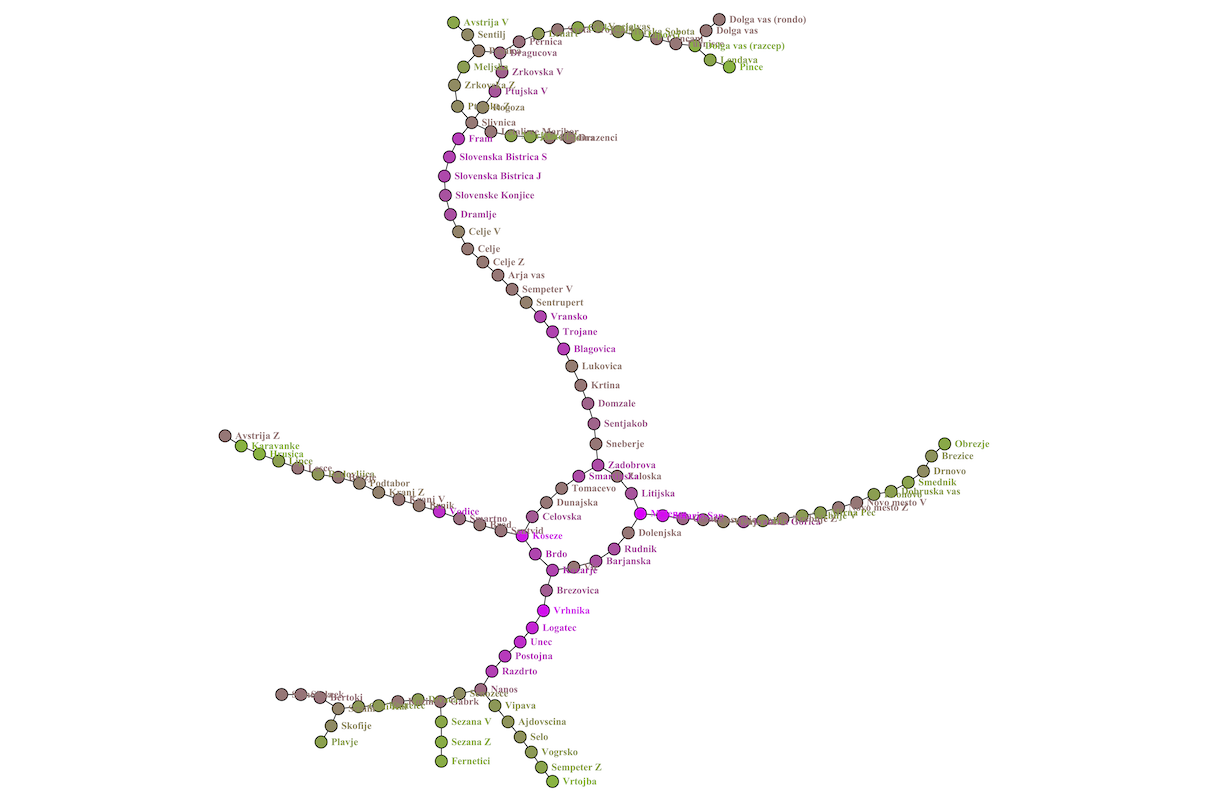
\includegraphics[width=0.66\textwidth]{highways}
	\caption{{\bf Slovenian highways network with node colors corresponding to traffic loads}}
	\label{fig:highways}
\end{figure}

\subsection*{What to submit?}

\paragraph{} State correlation coefficients and briefly discuss each result \points{3\times 0.25}. List top ten locations according to your best measure \points{0.25} and give brief interpretation \points{0.25}. Print out any code you might have used or describe how you solved the exercise \points{0.25}.

\bibliographystyle{alpha}
\bibliography{../misc/bibliography}

\end{document}
